% VESTA, CoMeSySo 2026, Springer LNNS.
\PassOptionsToPackage{expansion=false}{microtype}
\documentclass{llncs}
\usepackage[T1]{fontenc}
\usepackage[utf8]{inputenc}
\usepackage{graphicx}
\usepackage{booktabs}
\usepackage{array}
\usepackage{amsmath,amssymb}
\usepackage{url}
\usepackage{lmodern}

\urlstyle{same}

\begin{document}
\pagestyle{plain}
\mainmatter
\title{VESTA: Evaluating Time-Budgeted Multimodal Briefing for BIST Retail Users}
\titlerunning{VESTA: Time-Budgeted Multimodal Briefing}
\author{Peri Gunes\inst{1} \and Ozge Zelal Kucuk\inst{2} \and Harun Benli\inst{1}}
\authorrunning{P. Gunes et al.}
\institute{R\&D Center, Infina Software Development Inc., Istanbul, T\"urkiye\\
\email{pgunes@infina.com.tr}, \email{hbenli@infina.com.tr}
\and
Software Development Faculty, \.{I}stanbul Ayd{\i}n University, Istanbul, T\"urkiye\\
\email{ozelalkucuk@stu.aydin.edu.tr}}
\maketitle

\begin{abstract}
Retail investors on Borsa Istanbul (BIST) read KAP list text and charts under a short clock. VESTA evaluates that setting. Same-day KAP list teasers become a 16-d bag; a 40-bar candlestick is read together with the OHLCV numbers; a declared 1-, 3- or 10-minute budget changes how many tokens are shown while the mixer stays fixed. A $2\sigma$ realized-vol flag on the same day's OHLCV is recovered at 100\% F1 by a closed-form rule, so the headline task is next-day BIST100 direction. Score-space mixers and a learned Arevalo GMU ($W_v,W_t,W_z$ on raw 16-d text and the $24\times24$ image) are reported on public BIST100 data (2018 to 2026). No score-space mixer beats score-space GMU on seed 0 (minimum McNemar $p=0.46$); learned GMU does not either ($p=0.29$). Five-seed accuracy remains compatible with the majority prior (mean fusion $53.0\pm2.2$ versus $52.3$). T1/T3/T10 change coverage and templated length, not next-day accuracy (T3 and T10 both 49.7\% on seed 0). A long/short overlay loses to buy-and-hold on the 2025 to 2026 bull test window. Human NASA-TLX responses are not claimed. The replication package accompanies the submission.

\keywords{Econometrics \and Computational intelligence \and Decision support \and Multimodal fusion \and Borsa Istanbul}
\end{abstract}

\section{Introduction}
Retail investors sit between the textual density of the Public Disclosure Platform (KAP)~\cite{kap2026} and the visual flux of technical charts. The difficulty is not only volume but modality mismatch: a constructive disclosure can coincide with a failed breakout, and the two streams must be reconciled before a decision. Conventional DSS pipelines keep NLP and computer vision apart. A second failure mode is temporal: systems emit the same information density whether the user has sixty seconds or ten minutes~\cite{eppler2004overload,miller1956magical,sweller1988cognitive}. On a mobile-first retail platform that mismatch adds intrinsic load~\cite{sweller2023clt}.

FinMem layers trading-agent memory by information half-life~\cite{yu2024finmem}. VESTA scores a briefing whose clock is 1, 3 or 10 minutes: KAP list text and a 40-bar chart. The fusion rule does not change with the clock; only how many tokens are shown. T3 and T10 attach an M3 day-level hop; that analogue does not enter the mixer. Decision support is scored on next-day BIST direction, not on a realized-volatility flag that can be read off the same day's OHLCV table. Whenever a chart encoder is used, a numeric OHLCV baseline is reported beside it~\cite{jiang2023reimagining}. The public tables mix unimodal class scores with GMU~\cite{arevalo2017gmu}, tensor fusion~\cite{zadeh2017tfn} and a scalar gate, and they add one learned-GMU row that fits Arevalo's $W_v,W_t,W_z$ on the raw vectors. Actionability is a long/short overlay against buy-and-hold. The public chart is bars $t-40,\ldots,t-1$. A 12-participant NASA-TLX protocol is specified in \texttt{study/}; responses are not collected.

VESTA is the measurement protocol, not a proposed fusion rule. Time budgets T1, T3 and T10 change how many tokens are shown; the mixer is held fixed. The $2\sigma$ realized-vol flag on the same day's OHLCV is recovered at 100\% F1 by a closed-form rule, so the headline label is next-day direction. Tiers report coverage, declared latency, tokens and length-normalized noise; they do not raise next-day accuracy. Action is a long/short overlay against buy-and-hold on the 2025--2026 bull window. Table~\ref{tab:win2} is a 2023 holdout on the same index and does not reverse that claim. Score-space mixers are not separable from score-space GMU on seed 0 (minimum McNemar $p=0.46$); learned GMU is not either ($p=0.29$). Following Harvey et al.~\cite{harvey2016and} those comparisons are controls, not a ranking.

\subsection{Related work}
Financial NLP has moved from sentiment scoring~\cite{sohangir2018big} to domain LLMs such as FinGPT~\cite{yang2023fingpt}. Hallucination on prices remains a documented failure mode~\cite{kang2023deficiency}, so public text here is KAP list teasers, not free generation~\cite{lewis2020rag}. Tool-using agents~\cite{yao2023react} and FinMem~\cite{yu2024finmem} are the closest named relatives; this paper scores a briefing, not a trading agent. The public hop is M3 day-level cosine, not a portfolio retrieve-then-generate loop.

\subsection{Multimodal fusion and chart understanding}
GMU learns a multiplicative gate between modalities~\cite{arevalo2017gmu}; Tensor Fusion Networks use an outer product~\cite{zadeh2017tfn}; MulT uses directional pairwise cross-modal attention~\cite{tsai2019mult}. Jiang and Ji add a forget-gate over cross-modal attention maps~\cite{jiang2022cmga}. Public tables mix unimodal class scores with GMU, TFN, a scalar gate, mean, concat and one CPU attention layer. That layer is not the MulT of Tsai et al.: projections are frozen and there is a single head. A learned-GMU row fits Arevalo's maps on the raw vectors.

Pix2Struct and MatCha pretrain screenshot-to-text models~\cite{lee2023pix2struct,liu2023matcha}. Jiang, Kelly and Xiu show that CNNs on price-trend images extract return-predictive patterns~\cite{jiang2023reimagining}. That result requires a tabular OHLCV baseline beside any chart encoder. Akturk et al.\ forecast BIST100 from numeric indicators~\cite{akturk2026bist}; those features are the control whenever a chart encoder is scored.

\subsection{Cognitive load}
Presented density should match working-memory limits~\cite{sweller1988cognitive,sweller2023clt,miller1956magical,eppler2004overload}. Adaptive interfaces are judged by the task, not by whether a widget changed~\cite{gajos2006exploring,findlater2009adaptive}. Length-blind summarization metrics reward brevity~\cite{sun2019compare}, which is why Table~\ref{tab:tiers} reports $\mathrm{IN}_{\mathrm{new}}$ on delivered tokens. That table is a payload count. It is not a human-load result. The NASA-TLX protocol is Sect.~\ref{sec:user}; this manuscript has no responses.

\section{Methods}
\label{sec:methods}
Methods cover the pipeline, the mixers, time-budgeted delivery, and the evaluation design. VESTA has three layers (Fig.~\ref{fig:arch}). Perception uses a text module and a chart module; an off-the-shelf block mixes them; a temporal layer spends the user's time budget.

\begin{figure}[t]
\centering
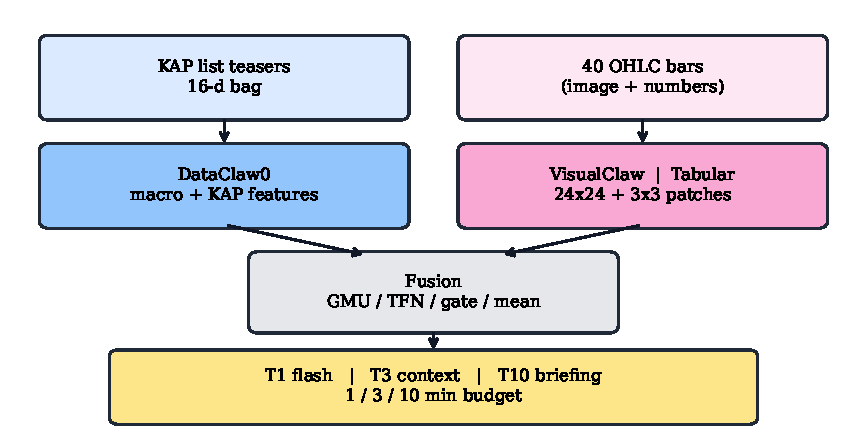
\includegraphics[width=0.88\textwidth]{figures/architecture.pdf}
\caption{Public path: KAP list bag and a 40-bar chart go through a mixer; T1, T3 or T10 spends the 1-/3-/10-minute budget.}
\label{fig:arch}
\end{figure}

\subsection{DataClaw0: text brief}
\label{sec:dataclw}
The public mixer path is a 16-d macro+KAP bag plus a templated brief. The retrieve-score hop is executed on cached BGE-M3 KAP-day vectors~\cite{chen2024m3,lewis2020rag,yao2023react}. $\alpha=1$. The $\beta$ gold / USD/TRY / session terms are not fitted and are not used. There is no user portfolio.

For each test day the hop is the prior KAP day with the highest cosine to that day's M3 vector. A same-date XU100 constituent with a KAP teaser is recorded as a peer hop. The retrieved analogue does not enter the 16-d mixer. T3 and T10 still spend a \texttt{hist\_analog} token; the console attaches the retrieved date and teaser.

The text dataset is VESTA-Public: one row per ticker-day (37{,}046 events; 27 BIST names plus XU100; 24 May 2018 to 19 August 2026). A row is kept if the name moved at least 2\%, the vol flag fired, RSI was extreme, or a KAP list item was published that calendar day. 19{,}645 rows have a same-day KAP teaser; 15{,}212 have a cached public HTML body. Yahoo headlines exist for 41 rows. Table~\ref{tab:text} lists four KAP strings in calendar order. A Turkish/English lexicon plus subject priors (dividend and buyback tilt bullish; fine and probe tilt bearish) yields $\mathrm{kap\_polarity}$. The same strings, plus USD/TRY, gold and the session, become an eight-plus-eight feature vector for the mixers. MiniLM~\cite{reimers2019sentence} and BGE-M3 embed the concatenated list text. The silver event-row brief for BIMAS on 2018-06-14, rebuilt from the stored columns, is: ``2018-06-14 BIMAS.IS. Session return +6.33\%. USD/TRY +1.65\%, gold +0.55\%. Ann. realized vol 33.8\%, RSI 48. Brief polarity bullish; chart cue none. Payların Geri Alınmasına İlişkin Bildirim. 13 Haziran 2018 Tarihli Pay Geri Alım İşlemleri''. That string is the ticker-day record, not the T10 token bag.

\begin{table}[t]
\caption{Example KAP list teasers in VESTA-Public (subject plus short summary from kap.org.tr), in calendar order. KAP pol.\ is $\mathrm{kap\_polarity}$, the KAP-only silver codebook, not mixed $\mathrm{text\_polarity}$.}
\label{tab:text}
\centering
\footnotesize
\begin{tabular}{@{}ll>{\raggedright\arraybackslash}p{6.1cm}l@{}}
\toprule
Date & Ticker & KAP list teaser & KAP pol.\ \\
\midrule
2018-05-25 & YKBNK & Özel Durum Açıklaması (Genel). Bankamıza verilen idari para cezasının iptaline ilişkin açılan dava hk. & bearish \\
2018-06-14 & BIMAS & Payların Geri Alınmasına İlişkin Bildirim. 13 Haziran 2018 Tarihli Pay Geri Alım İşlemleri & bullish \\
2018-06-19 & ASELS & BISTECH Pay Piyasası Alım Satım Sistemi Duyurusu. Temettü Ödemesi & bullish \\
2020-08-11 & FROTO & Özel Durum Açıklaması (Genel). Rekabet Kurulu Soruşturma Kararı Hakkında & bearish \\
\bottomrule
\end{tabular}
\end{table}

\subsection{VisualClaw: candles, pixels, tokens}
\label{sec:vision}
VisualClaw draws the chart from OHLC bars. Figure~\ref{fig:vision} is one XU100 window from the test split.
\begin{enumerate}
\item Take the 40 sessions strictly before day $t$ (open, high, low, close). Today's candle is not in the picture.
\item Paint a grayscale candlestick: a one-pixel wick and a rectangular body. Close $\ge$ open is dark ($30/255$); close $<$ open is light ($180/255$). Price is min-max scaled to that window.
\item Resize to $24\times24$. The vision MLP flattens this to a $576$-d vector and classifies with hidden layers $64$-$32$. That is the vision row in Table~\ref{tab:fwd}.
\item For the 1-layer attention mixer only, cut the same $24\times24$ image into a $3\times3$ grid of $8\times8$ patches (nine visual tokens). The $16$-d text brief is split into two tokens. Projections are frozen (seed 0); only the MLP on top is trained.
\end{enumerate}
Two further probes sit beside the mixer: a frozen ImageNet ViT-B/16~\cite{dosovitskiy2021vit} that resizes a colour chart to $224\times224$ and uses that model's own $16\times16$ patches; and zero-shot DePlot / MatCha, which see a matplotlib RGB screenshot of the same 40 bars (Fig.~\ref{fig:vision}(a)). Tabular OHLCV at day $t$ is always reported beside the picture~\cite{jiang2023reimagining}. Public tables train the flattened $24\times24$ MLP; they do not add a recency term to patch positions.

\begin{figure}[t]
\centering
\begin{minipage}[b]{0.50\textwidth}
\centering
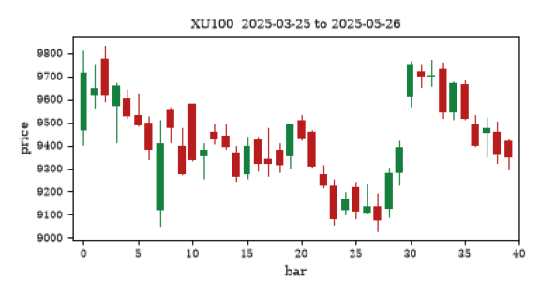
\includegraphics[width=\linewidth]{figures/visualclaw_a.pdf}\\[0.35em]
\small (a)~RGB screenshot (DePlot / MatCha)
\end{minipage}\hfill
\begin{minipage}[b]{0.23\textwidth}
\centering

\includegraphics[width=\linewidth]{figures/visualclaw_b.pdf}\\[0.35em]
\small (b)~$24\times24$ MLP tensor
\end{minipage}\hfill
\begin{minipage}[b]{0.23\textwidth}
\centering
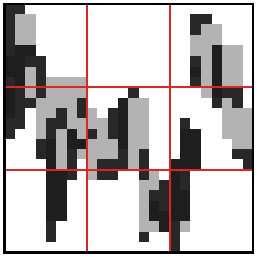
\includegraphics[width=\linewidth]{figures/visualclaw_c.pdf}\\[0.35em]
\small (c)~Nine $8\times8$ tokens (1-layer attention)
\end{minipage}
\caption{VisualClaw on one XU100 test window (40 bars before 27 May 2025). (a)~RGB screenshot for DePlot / MatCha. (b)~$24\times24$ grayscale tensor the MLP flattens. (c)~Nine $8\times8$ tokens for the 1-layer attention mixer.}
\label{fig:vision}
\end{figure}

\subsection{Fusion}
\label{sec:fusion}
Arevalo et al.\ write the bimodal GMU as~\cite{arevalo2017gmu}
\begin{align}
h_v&=\tanh(W_v x_v),\qquad h_t=\tanh(W_t x_t),\label{eq:gmuh}\\
z&=\sigma(W_z[x_v;x_t]),\qquad h=z\,h_v+(1-z)\,h_t,\label{eq:gmu}
\end{align}
so $z$ near 1 keeps the visual branch. Zadeh et al.\ flatten $[h_t;1]\otimes[h_v;1]$ (TFN)~\cite{zadeh2017tfn}. Table~\ref{tab:fwd} has two GMU rows. The score-space GMU takes unimodal class-score vectors as $x_t$ and $x_v$ and sets $z$ from the score gap (Arevalo's mix; $W_v,W_t,W_z$ unused in that row only). The learned-GMU row fits those three maps on the raw 16-d text vector and the flattened $24\times24$ image by minibatch gradient descent, then a linear head on $h$. The TFN row uses the outer product on the same class scores. The scalar-gate row uses
\begin{align}
g&=\sigma\bigl(4(p_{\mathrm{text}}-p_{\mathrm{vision}})\bigr),\label{eq:gate}\\
h&=g\,\tanh(p_{\mathrm{text}})+(1-g)\,\tanh(p_{\mathrm{vision}}),\label{eq:fuse}
\end{align}
so $g$ near 1 keeps text. A small MLP reads the mix. Mean and concat are unweighted. The 1-layer attention row is one CPU attention layer on two text tokens and nine $8\times8$ patches, with frozen projections. That layer is not Tsai MulT~\cite{tsai2019mult}. The fused call drives T1 / T3 / T10.

\subsection{Temporal Orchestration Layer}
\label{sec:tol}
The user's clock $B\in\{1,3,10\}$ minutes is the intended independent variable. No participant sat that cap. Table~\ref{tab:tiers} reports declared latencies 0.9 / 2.1 / 3.4\,s, not wall-clock. T3 and T10 emit the same fused call; extra tokens are templates.
\begin{itemize}
\item T1 (flash). Emit a gated alert only if $|g-0.5|>\tau$ with $\tau=0.18$; otherwise abstain. Declared latency 0.9\,s.
\item T3 (context). Always emit the fused call plus a retrieved analogue token (M3 cosine, $\alpha=1$; no portfolio).
\item T10 (briefing). Expand into a macro explanation and a hedge sketch (e.g.\ airline exposure versus a gold certificate). The 3.4\,s figure in Table~\ref{tab:tiers} is a declared budget, not measured wall-clock.
\end{itemize}
The mixer stays fixed. Tiers change how many tokens are shown. Section~\ref{sec:tiers} reports coverage, latency, tokens and noise per tier.

\subsection{Evaluation protocol}
\label{sec:protocol}
The evaluation has a leakage diagnostic, a primary next-day direction task, per-tier delivery metrics, and a paper-trading overlay.

\subsubsection{Diagnostic: the realized-volatility label}
\label{sec:leak}
The $2\sigma$ realized-vol flag at day $t$ is 20-day realized vol (annualized) above the 60-day rolling mean plus $2\sigma$ of that 20-day vol series, all taken from the tabular vector at $t$ (100\% F1). The public chart does not contain today's candle, so vision F1 on this label is lag-1 recovery. We report the flag only as a diagnostic.

\subsubsection{Primary task: forward direction}
The primary label at close of day $t$ is the next session's direction: $y_{t+1}=1$ if the BIST100 simple return $r_{t+1}$ is positive, and $y_{t+1}=0$ otherwise. The label is unknown at the close of day $t$. We also report a five-session horizon. Splits are chronological (70/15/15) to block look-ahead~\cite{akturk2026bist}.

\subsubsection{Metrics}
\label{sec:metrics}
Classification. Accuracy and macro-F1, mean $\pm$ $1.96$ standard error over five seeds. McNemar with continuity correction~\cite{dietterich1998approx} on seed 0 of one chronological holdout. Table~\ref{tab:fwd} has fourteen rows. Pairwise McNemar versus score-space GMU is a control, not a winner (minimum $p=0.46$ for score-space mixers; $p=0.29$ for learned GMU). With that many rows we follow Harvey et al.~\cite{harvey2016and} and do not pick a winner after an uncorrected search.

Sentiment / technical accuracy. Table~\ref{tab:proxy} in Sect.~\ref{sec:exp} reports proxy accuracy versus next-day direction. Macro flags and KAP polarity are deterministic rules on one chronological split (no seed CI). Vision and tabular are five-seed means from Table~\ref{tab:fwd}. Three KAP codebooks on the 10k slice give Fleiss $\kappa=0.50$; there are no human annotators. Chart A/B Cohen $\kappa=0.52$~\cite{cohen1960kappa}. The 250-row sample has no annotators; those columns are codebook B.

Information noise. This is the computational cognitive measure. Let $N_{\mathrm{raw}}$ be tokens in the unprocessed window (the raw KAP list plus session flags) and $N_{\mathrm{del}}$ tokens actually delivered in the T1, T3 or T10 briefing. Let $N_{\mathrm{irrel}}$ be delivered tokens that are not in a relevance lexicon for that window (session, USD/TRY, gold, vol, KAP digest). The index $\mathrm{IN}_{\mathrm{old}}=N_{\mathrm{irrel}}/N_{\mathrm{raw}}$ rewards short answers: a 40-token briefing that is 80\% filler still looks clean against a 700-token feed~\cite{sun2019compare}. We therefore report
\begin{equation}
\mathrm{IN}_{\mathrm{new}}=N_{\mathrm{irrel}}/N_{\mathrm{del}},
\label{eq:innew}
\end{equation}
the fraction of the delivered finance briefing that is non-actionable, together with the compression ratio $N_{\mathrm{del}}/N_{\mathrm{raw}}$. $\mathrm{IN}_{\mathrm{new}}$ is our index; Sun et al.\ motivate dividing by delivered length. Both counts use templated token bags with filler padding, so $\mathrm{IN}_{\mathrm{new}}$ rises by construction when T3/T10 add filler. Table~\ref{tab:tiers} is that computational proxy; human NASA-TLX is unreported (Sect.~\ref{sec:user}).

Decision quality. Classification F1 does not say whether acting on the output helps~\cite{findlater2009adaptive}. We paper-trade a long/short overlay: $+1$ if the model predicts up, $-1$ otherwise, with 5\,bp round-trip cost, and compare Sharpe, total return and max drawdown to buy-and-hold. Table~\ref{tab:bt} is that control; Sect.~\ref{sec:user} is the human cognitive protocol.

\subsubsection{Public replication corpus}
Numbers below use VESTA-Public: XU100.IS, USDTRY and COMEX gold from 24 May 2018 to 19 August 2026 (2{,}052 index windows after a 40-day lookback; test $n=308$ from 27 May 2025), 27 BIST names, and the public KAP list inventory of 39{,}890 filings (27 names; scrape window 2 January 2018 to 27 August 2026). Tables~\ref{tab:proxy} to~\ref{tab:bt} are index-level; the 37{,}046-row event panel also labels constituents. KAP-only polarity: 7{,}172 / 3{,}742 / 26{,}132 (bullish / bearish / neutral); 15{,}212 rows have a cached public HTML body. Mixers use the 16-d macro+KAP vector; MiniLM and BGE-M3 are unimodal text probes on the same list teasers.

\subsection{Human protocol}
\label{sec:user}
The computational load numbers sit with the tier table in Sect.~\ref{sec:tiers}. A BIST retail user on a mobile desk has about one, three or ten minutes between a KAP drop and an order. That clock is the independent variable. The dependent quantities are coverage (how often the system speaks), declared latency, tokens delivered, and $\mathrm{IN}_{\mathrm{new}}$ (what fraction of the delivered briefing is non-actionable). The token bags are built from the day's finance flags: session return, USD/TRY, gold, realized vol, a KAP digest, and, on T3/T10, a historical analogue and a hedge sketch. Those counts measure load on the payload. They do not measure load on a person~\cite{gajos2006exploring,findlater2009adaptive}.

The human protocol is in \texttt{study/}. Twelve participants would see eight sealed snapshots from the public test window (two XU100 sessions and six constituents: SASA, SISE, YKBNK, TAVHL, AKBNK, PETKM), within subject. The sealed gold is the subsequent week's realized direction of that name. Conditions are the raw KAP+OHLC feed, a unimodal text or chart, or the matching VESTA tier, under a 1-, 3- or 10-minute cap. Outcomes are the week-direction call, time-to-decision, NASA-TLX, and a 7-point trust item. Consent and the bilingual instrument are in \texttt{study/}.

Responses have not been collected ($n=0$). This paper does not claim a human-load or trust result. A model dry-run on the sealed gold hits $4/8$ name-level weeks for the raw session sign; index mixers are scored only on the two XU100 weeks (text $0/2$, gated $1/2$). NASA-TLX and trust stay blank. The executable protocol remains in \texttt{study/} so a later sample can be scored against the same gold.

\section{Results}
\label{sec:exp}
Unimodal encoders are sklearn MLPs (64-32, Adam, early stopping) on standardized features. Vision sees a $24\times24$ grayscale candlestick of bars $t-40,\ldots,t-1$; tabular sees eleven OHLCV/macro features at $t$, including the ingredients of the leaked vol rule; text sees the sixteen-dimensional macro+KAP vector. Five seeds $\{0,\ldots,4\}$. Training is on CPU. Public BGE-M3 and frozen ViT-B/16 are unimodal probes; they remain unimodal in Table~\ref{tab:fwd}.

\subsection{Proxy accuracy}
Table~\ref{tab:proxy} is the rule and encoder proxy against next-day direction. Macro flags are the strongest single-split rule (54.9\%). KAP polarity on list teasers is 49.7\%. The $24\times24$ vision MLP and tabular OHLCV repeat their five-seed means from Table~\ref{tab:fwd}.

\begin{table}[t]
\caption{Proxy accuracy versus next-day direction $y_{t+1}$ (test $n=308$). Macro/KAP are single-split rules; vision/tabular are mean $\pm$ $1.96$ se over five seeds.}
\label{tab:proxy}
\centering
\begin{tabular}{lc}
\toprule
Proxy & Acc.\ (\%) \\
\midrule
Macro flags (USD/TRY, gold, vol, shock) & $54.9$ \\
Vision $24\times24$ MLP & $52.9\pm2.3$ \\
Tabular OHLCV & $50.6\pm0.0$ \\
KAP polarity (lexicon on public list text) & $49.7$ \\
\bottomrule
\end{tabular}
\end{table}

\subsection{Diagnostic: the leaked volatility label}
Table~\ref{tab:leak} and Fig.~\ref{fig:leak} confirm the closed-form critique. The $2\sigma$ rule on the tabular vector scores 100\% F1. A tabular MLP that is given those numbers reaches 96.8\% accuracy (macro-F1 86.6\%; the F1 drop is class imbalance: 25 positives among 308 test days, 8.1\%; 9.4\% of all 2{,}052 windows). The $24\times24$ vision encoder, which never sees day $t$'s candle, falls to 90.6\% accuracy and 58.2\% F1.

\begin{table}[t]
\caption{Diagnostic task: $2\sigma$ realized-vol label, computable from the tabular vector at $t$. The closed-form row is a single split. MLP rows are mean $\pm$ $1.96$ se over five seeds. Vision sees bars $t-40,\ldots,t-1$ only.}
\label{tab:leak}
\centering
\begin{tabular}{lcc}
\toprule
Method & Accuracy (\%) & Macro-F1 (\%) \\
\midrule
Closed-form OHLCV rule & $100.0$ & $100.0$ \\
Tabular MLP (same numbers) & $96.8\pm0.0$ & $86.6\pm0.0$ \\
Vision MLP (chart image) & $90.6\pm1.1$ & $58.2\pm3.0$ \\
\bottomrule
\end{tabular}
\end{table}

\begin{figure}[t]
\centering
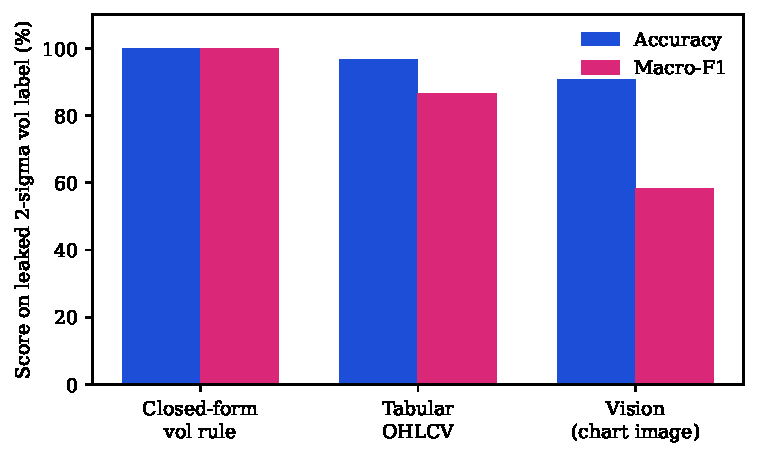
\includegraphics[width=0.62\textwidth]{figures/leakage.pdf}
\caption{Diagnostic $2\sigma$-vol label. The closed-form OHLCV rule scores 100\% F1; the chart omits day $t$.}
\label{fig:leak}
\end{figure}

\subsection{Primary task: next-day direction}
Five-seed accuracy CIs overlap the majority prior 52.3\%. Mean fusion $53.0\pm2.2$ is not a winner. Table~\ref{tab:fwd} reports the leakage-free task (test prior 52.3\% up-days). Accuracy / macro-F1: text-only (macro$+$KAP) $52.1\pm2.4$ / $47.3\pm1.5$ against majority $52.3$ / $34.3$; MiniLM $53.0\pm0.4$ / $50.7\pm1.9$; public BGE-M3 $51.1\pm1.9$ / $50.2\pm2.1$; frozen ViT-B/16 $50.9\pm1.4$ / $50.3\pm1.6$. Mixers share 16-d text and the $24\times24$ image. Among score-space mixers, none beats score-space GMU on seed 0 (minimum McNemar $p=0.46$). Learned GMU ($W_v,W_t,W_z$ on the raw vectors) is $52.5\pm0.5$ / $40.3\pm4.4$ and does not beat score-space GMU either (seed-0 McNemar $p=0.29$); the F1 drop is majority collapse. On the five-session horizon (seed 0) tabular accuracy / F1 is 59.1\% / 39.9\%; vision is 51.9\% / 49.0\% and the scalar gate is 50.3\% / 49.3\%.

\begin{table}[t]
\caption{Next-day BIST100 direction on VESTA-Public (test $n=308$). Mean $\pm$ $1.96$ se, five seeds. MiniLM, BGE-M3 and ViT are unimodal probes. Mixers include 1-layer attention, GMU~\cite{arevalo2017gmu} and TFN~\cite{zadeh2017tfn}. Score-space GMU/TFN/gate mix unimodal class scores. Learned GMU fits Arevalo's $W_v,W_t,W_z$ on raw text and the $24\times24$ image. The 1-layer attention row is a single frozen-projection head, not Tsai et al.'s MulT.}
\label{tab:fwd}
\centering
\footnotesize
\setlength{\tabcolsep}{3.5pt}
\begin{tabular}{lcc}
\toprule
Configuration & Accuracy (\%) & Macro-F1 (\%) \\
\midrule
Mean fusion & $53.0\pm2.2$ & $52.4\pm2.3$ \\
Text-only (MiniLM KAP) & $53.0\pm0.4$ & $50.7\pm1.9$ \\
Vision-only ($24\times24$ MLP) & $52.9\pm2.3$ & $51.4\pm2.6$ \\
Concatenation & $52.8\pm1.8$ & $51.1\pm2.3$ \\
Learned GMU ($W_v,W_t,W_z$) & $52.5\pm0.5$ & $40.3\pm4.4$ \\
Majority class & $52.3\pm0.0$ & $34.3\pm0.0$ \\
TFN & $52.1\pm2.1$ & $51.7\pm2.1$ \\
Text-only (macro + KAP) & $52.1\pm2.4$ & $47.3\pm1.5$ \\
Scalar gate (score-space) & $51.8\pm1.7$ & $51.4\pm1.8$ \\
Text-only (public BGE-M3) & $51.1\pm1.9$ & $50.2\pm2.1$ \\
Vision-only (frozen ViT-B/16) & $50.9\pm1.4$ & $50.3\pm1.6$ \\
GMU (score-space) & $50.6\pm2.4$ & $50.6\pm2.4$ \\
Tabular OHLCV & $50.6\pm0.0$ & $41.8\pm0.0$ \\
1-layer attention & $50.2\pm3.1$ & $48.4\pm3.0$ \\
\bottomrule
\end{tabular}
\end{table}

\begin{figure}[t]
\centering
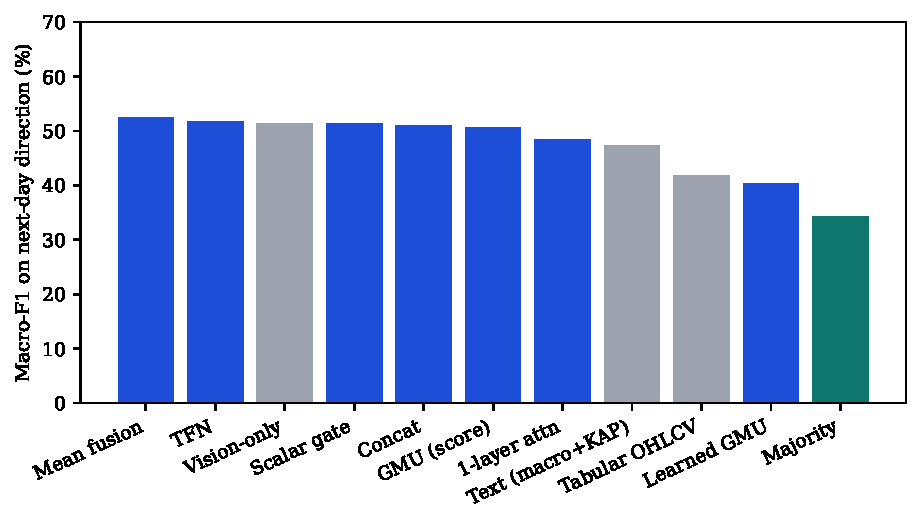
\includegraphics[width=0.92\textwidth]{figures/forward_f1.pdf}
\caption{Macro-F1 for score-space mixers, sklearn unimodal rows, and learned GMU from Table~\ref{tab:fwd}, in the same row order. MiniLM, BGE-M3 and ViT stay in the table only. Mean $\pm$ $1.96$ se is in the table.}
\label{fig:fwd}
\end{figure}

Replacing the gate with a fixed mean changes five-seed F1 from $51.4\pm1.8$ to $52.4\pm2.3$ (seed-0 McNemar $p=1.00$).

\subsection{Zero-shot Pix2Struct and MatCha}
\label{sec:vlm}
Zero-shot DePlot~\cite{lee2023pix2struct} and MatCha-ChartQA~\cite{liu2023matcha} run on CPU matplotlib screenshots of the full test window ($n=308$), with no fine-tune. Calls are $\mathrm{sign}(\hat{y}_{\mathrm{last}}-\hat{y}_{\mathrm{first}})$. Table~\ref{tab:vlm} also scores the numeric window trend of the input OHLC, which is still not $y_{t+1}$. DePlot parses 307/308 images and recovers that trend on 77.9\% of days; next-day accuracy is 52.9\%. MatCha-ChartQA often returns the bar index (parse rate 166/308) and matches the majority class on $y_{t+1}$.

\begin{table}[t]
\caption{Zero-shot CPU screenshot VLMs on the full test window ($n=308$), with no fine-tune.}
\label{tab:vlm}
\centering
\setlength{\tabcolsep}{3.5pt}
\begin{tabular}{lccc}
\toprule
Method & Acc.\ vs $y_{t+1}$ & Macro-F1 & Acc.\ vs window trend \\
\midrule
DePlot (Pix2Struct) & $52.9$ & $51.9$ & $77.9$ \\
MatCha-ChartQA & $52.3$ & $46.0$ & $58.4$ \\
Majority & $52.3$ & $34.3$ & n/a \\
Numeric window trend & $51.6$ & $49.5$ & $100.0$ \\
\bottomrule
\end{tabular}
\end{table}

\subsection{Per-tier measurement}
\label{sec:tiers}
Table~\ref{tab:tiers} and Fig.~\ref{fig:tiers} measure the Temporal Orchestration Layer. Latencies 0.9 / 2.1 / 3.4\,s are declared budgets, not wall-clock. No participant sat the 1-/3-/10-minute cap. On seed 0, T1 covers 32.5\% of days (60.0\% among emitted calls; 55.2\% after majority fill). T3 and T10 always emit (coverage 100\%). T3 accuracy equals T10 accuracy (both 49.7\%) because extra tokens are templates, not new evidence. The M3 hop retrieves on all 308 test days (mean cosine 0.89). The retrieved day's next-day sign matches $y_{t+1}$ on 49.8\% of 305 scored days. That analogue does not beat the majority prior, and it does not enter the mixer. $\mathrm{IN}_{\mathrm{old}}<7\%$ for every tier. $\mathrm{IN}_{\mathrm{new}}$ is 60.3 / 82.1 / 93.6\%; that series is the padding index. It rises by construction when T3/T10 add filler.

\begin{table}[t]
\caption{Temporal Orchestration Layer on seed 0. Latency is a declared budget, not measured GPU time. Acc.\ is among emitted calls; T1 overall accuracy with majority fill is 55.2\%.}
\label{tab:tiers}
\centering
\setlength{\tabcolsep}{3.5pt}
\begin{tabular}{lcccccc}
\toprule
Tier & Cov. (\%) & Lat. (s) & Acc. (\%) & Tokens & $\mathrm{IN}_{\mathrm{old}}$ & $\mathrm{IN}_{\mathrm{new}}$ \\
\midrule
T1 flash & 32.5 & 0.9 & 60.0 & 6 & 0.5\% & 60.3\% \\
T3 context & 100.0 & 2.1 & 49.7 & 17 & 1.9\% & 82.1\% \\
T10 briefing & 100.0 & 3.4 & 49.7 & 52 & 6.8\% & 93.6\% \\
\bottomrule
\end{tabular}
\end{table}

\begin{figure}[t]
\centering
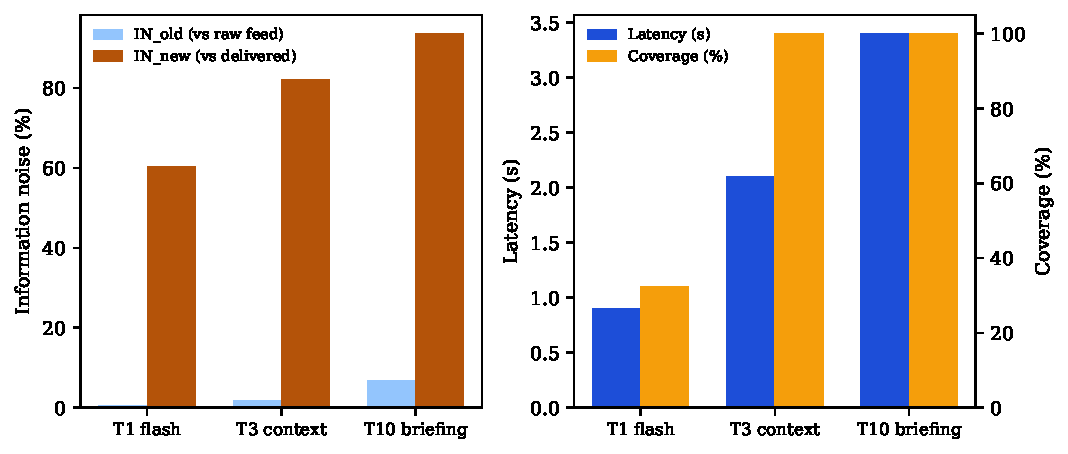
\includegraphics[width=0.86\textwidth]{figures/tiers.pdf}
\caption{Left: length-normalized noise of the delivered briefing ($\mathrm{IN}_{\mathrm{old}}$ versus $\mathrm{IN}_{\mathrm{new}}$). Right: declared latency and coverage for T1, T3 and T10.}
\label{fig:tiers}
\end{figure}

\subsection{Decision quality}
Table~\ref{tab:bt} reports the paper-trading overlay. In the May 2025 to August 2026 test window, BIST100 buy-and-hold returned $+56.3\%$ (Sharpe 1.69). Every seed-0 overlay we tried underperformed that long-only benchmark after 5\,bp costs. Vision-only (Sharpe 0.37) and the scalar gate (0.33) were positive but far below BH; GMU and tabular were negative. A bull-market holdout is a hard test for a long/short overlay~\cite{harvey2016and}.

\begin{table}[t]
\caption{Paper-trading overlay on seed-0 calls, one bull chronological window (27 May 2025 to 19 August 2026), 5\,bp costs. BH is long-only BIST100. Dir.\ is the fraction of days the signed position matches $y_{t+1}$; for buy-and-hold that equals the up-day prior. Long/short versus BH is a hard test on this window. Table~\ref{tab:win2} is the earlier 2023 holdout on the same index.}
\label{tab:bt}
\centering
\begin{tabular}{lcccc}
\toprule
Policy & Dir.\ (\%) & Sharpe & Total ret. & Max DD \\
\midrule
Buy-and-hold & 52.3 & $1.69$ & $+56.3\%$ & $14.5\%$ \\
Vision-only overlay & 50.0 & $0.37$ & $+7.6\%$ & $16.4\%$ \\
Scalar-gate overlay & 49.7 & $0.33$ & $+6.3\%$ & $17.1\%$ \\
Tabular overlay & 50.6 & $-0.11$ & $-6.2\%$ & $23.0\%$ \\
GMU overlay & 48.1 & $-0.74$ & $-21.8\%$ & $27.4\%$ \\
\bottomrule
\end{tabular}
\end{table}

\subsection{Earlier holdout (2023)}
\label{sec:win2}
Table~\ref{tab:win2} is a second chronological cut on the same index, not a second market. Models are trained on days strictly before 2 January 2023 and scored on 2023 ($n=248$; prior 51.2\%). Five-seed mean fusion accuracy is $53.3\pm1.7$ against majority 51.2. On seed 0 the vision overlay beats buy-and-hold (Sharpe 1.81 versus 0.99). That does not reverse Table~\ref{tab:bt}: we do not name a winner after two uncorrected windows~\cite{harvey2016and}.

\begin{table}[t]
\caption{Earlier holdout on XU100, 2 January 2023 to 29 December 2023 ($n=248$). Train is all sessions before 2023-01-01 ($n=1149$). Accuracy is mean $\pm$ $1.96$ se over five seeds. Overlay Sharpe and return are seed 0, 5\,bp costs; n/a where that mixer has no overlay row. Buy-and-hold on the same window: Sharpe $0.99$, $+34.7$\%.}
\label{tab:win2}
\centering
\footnotesize
\setlength{\tabcolsep}{3.5pt}
\begin{tabular}{lcccc}
\toprule
Configuration & Acc.\ (\%) & Macro-F1 (\%) & Sharpe & Total ret.\ \\
\midrule
Mean fusion & $53.3\pm1.7$ & $51.3\pm2.8$ & n/a & n/a \\
Vision-only ($24\times24$ MLP) & $53.1\pm1.8$ & $50.6\pm2.9$ & $1.81$ & $+81.4\%$ \\
Scalar gate (score-space) & $52.5\pm1.7$ & $50.4\pm1.2$ & $1.64$ & $+70.6\%$ \\
Tabular OHLCV & $51.2\pm0.0$ & $34.6\pm0.0$ & $0.56$ & $+14.8\%$ \\
Majority class & $51.2\pm0.0$ & $33.9\pm0.0$ & n/a & n/a \\
Text-only (macro + KAP) & $50.4\pm1.3$ & $40.5\pm2.3$ & n/a & n/a \\
\bottomrule
\end{tabular}
\end{table}

\section{Discussions}
The public path runs an M3 day-level hop ($\alpha=1$, no portfolio). The analogue hit rate is 49.8\%; the hop does not enter the mixer. T3 and T10 both score 49.7\% on seed 0 because extra tokens are templates. Five-seed accuracy remains compatible with the majority prior. The 2025--2026 bull overlay loses to buy-and-hold; the 2023 holdout does not reverse that claim. Human NASA-TLX is unreported ($n=0$). Fleiss $\kappa=0.50$ is three codebooks; there are no human annotators. Public text is KAP list teasers, not full KAP HTML.

Learned GMU does not beat score-space GMU ($p=0.29$), and no score-space mixer does either (minimum $p=0.46$). The learned-GMU row is the control for fusing unimodal class scores. The public chart uses bars $t-40,\ldots,t-1$. Information noise and tier latencies are simulated. $\mathrm{IN}_{\mathrm{new}}$ rises by construction when T3/T10 add filler.

The 12-participant NASA-TLX study in \texttt{study/} has no responses, so human load and trust are unreported. There is no human-annotator gold set; polarity is silver codebook output. Full disclosure-detail pages are absent.

\subsubsection{Disclosure of Interests.} The authors declare that they have no competing interests relevant to the content of this article. P.G.\ and H.B.\ are employed by Infina Software Development Inc., which operates a BIST retail platform; the public replication does not use proprietary KAP text.

\bibliographystyle{splncs04}
\bibliography{vesta}

\end{document}
